\documentclass[
  % Replace twoside with oneside if you are printing your thesis on a single side
  % of the paper, or for viewing on screen.
  oneside,
  %twoside,
  11pt, a4paper,
  footinclude=true,
  headinclude=true,
  cleardoublepage=empty
]{scrbook}

\usepackage{python}
\usepackage[linedheaders,parts,pdfspacing,dottedtoc]{classicthesis}
%\usepackage[linedheaders,parts,pdfspacing]{classicthesis}
\usepackage[utf8]{inputenc}
\usepackage{graphicx}
\usepackage{amsmath}
\usepackage[margin=1in]{geometry}
\usepackage{indentfirst}
\usepackage{amsfonts}
\usepackage[english]{babel}
\usepackage{float}
%\usepackage[usenames,dvipsnames]{color}
\usepackage{lipsum}
\usepackage{amsthm}
\usepackage{acronym}
\usepackage{listings}
\usepackage{minted}
\usepackage{subfig}
\usepackage{url}

\setlength{\parindent}{4em}
\setlength{\parskip}{1em}
\def\UrlBreaks{\do\/\do-}

\begin{document}

\begin{titlepage}

\newcommand{\HRule}{\rule{\linewidth}{0.5mm}} 
\center 
 

\textsc{\LARGE University of Coimbra}\\[1cm]
\textsc{\large Department of Informatics Engineering}\\[.5cm]
\textsc{\large Masters Degree in Informatics Engineering}\\[4cm]
\textsc{\large Software Quality and Dependability}\\[1cm]


\HRule \\[0.5cm]
{\huge \bfseries Assignment 1}\\[0.4cm]
{\huge \bfseries N-Version Programming Web Services}\\[0.4cm]
\HRule \\[5cm]
 
\begin{minipage}{0.4\textwidth}
\begin{flushleft} \large
\emph{Author:}\\
João Miguel \textsc{Simões}  \\2011150045
\end{flushleft}
\end{minipage}
~
\begin{minipage}{0.4\textwidth}
\begin{flushright} \large
\emph{Author:} \\
Joaquim \textsc{Leitão}  \\2011150072
\end{flushright}
\end{minipage}\\[2cm]
~
\begin{minipage}{0.3\textwidth}
\begin{flushleft} \large
\emph{Author:} \\
Leonardo \textsc{Toledo}  \\2011168960
\end{flushleft}
\end{minipage}\\[2cm]

{\large \today}\\[3cm]

\vfill

\end{titlepage}

\begin{titlepage}

\newcommand{\HRule}{\rule{\linewidth}{0.5mm}}

\noindent
\HRule \\[0.05cm]
{\normalsize \bfseries \color{black}{EXECUTIVE SUMMARY}} \\[0.05cm]
\HRule \\[0.05cm]

    In critical systems one of the most important attributes is dependability. For this propose, this project explores the \emph{N-Version Programming} method to improve the reliability of an Insulin Dose Calculator. This is a real world problem where reliability of the result is a critical aspect.
    
    Applications that make use of \emph{N-Version Programming} techniques usually face the problem of, given a set of \emph{N} possibly different answers for the same problem, selecting the correct one to be considered by the application. To overcome this obstacle, a \emph{voting} system is used in such applications. The goal of this voter is to select which answer to be considered by the application, based on the set of answers given by each version considered. In short, its operation mode can be as simple as selecting the most common answer, since that would most probably be the correct value to be considered by the application.
    
    Furthermore, as the \emph{voter} is a critical aspect of N-Version programming, since it determines the choice the system will make regarding each version considered, a formal verification of this entity is usually done to assure the correct operation of this entity. A formal verifications of a given entity is performed under a simplified model of that entity, in which exhaustive testing is done, assuring the correct behaviour of the modelled system in all its possible states.
    
    If the created model operates according to what is expected in those tests, then if no errors are made converting that model to the \emph{"real"} implementation of the system, we can guarantee that specific system will operate as expected and agreed. This is particularly important in critical software applications, where the software produced must be tested to the limit.
    
    
    In our work we present an application that makes use of \emph{N-Version Programming} to compute the number of Insulin units to administrate to a given patient, based on a series of parameters specified. We also present one \emph{Web Service} that can be used as one of the \emph{N-Versions} to be considered in this scenario, and our concept and implementation of a \emph{Voter} system that selects the result presented to the user, based on the computations made by a series of \emph{Web Services}.

\end{titlepage}

%*******************************************************
% Table of Contents
%*******************************************************
\pdfbookmark[1]{\contentsname}{toc}
\setcounter{tocdepth}{2} % <-- 2 includes up to subsections in the ToC
\setcounter{secnumdepth}{3} % <-- 3 numbers up to subsubsections

\tableofcontents % help me, it stopped working for some god forsaken reason!

%*******************************************************
% List of Figures
%*******************************************************

%%%
%% Removed for now
%%%
%\pdfbookmark[1]{\listfigurename}{lof}

\listoffigures

\chapter{Introduction}

This document addresses the work developed by \emph{João Miguel Simões}, \emph{Joaquim Leitão} and \emph{Leonardo Toledo} as part of the first assignment of the \emph{Master's Degree in Informatics Engineering} \emph{Software Quality and Dependability} course.

In the present work, the development of a fully functional \emph{Web Service} based on \emph{N-Version} programming \emph{Insulin Dose Calculator} for patients with type-2 diabetes is proposed, as well as the development of a client interface for this system, aiming to ease its usage in an application scenario.

As studied and documented by medical specialists, type-2 diabetes patients need periodic insulin injections to help process blood sugar, thus, is it critical for such patients to obtain insulin in the right amount that allows them to metabolise the carbohydrates obtained from food.\footnote{It is even more critical to provide the right amount of insulin to the patient, since higher insulin administration doses may cause \emph{hypoglycemia}, possibly leading to coma and brain damage}.

Specialists have recommended that such patients seek to maintain a target glucose level somewhere between $80$ mg/dl and $120$ mg/dl throughout the day. To keep their glucose levels within the recommended values, type-2 diabetes patients regularly measure their blood glucose level and calculate the necessary insulin dose needed to inject in their bodies to process the excess blood sugar.

These patients inject regularly a certain number of \emph{insulin units} throughout the day, adding up to a \emph{daily insulin total number of units}. Part of this total is intended to cover the background insulin needed between meals, and is called \emph{basal insulin replacement}. The remaining, called \emph{bolus insulin replacement} is needed after every meal to process the carbohydrates obtained from food.

The main goal of the \emph{Insulin Dose Calculator} proposed in this assignment is to calculate and indicate the patient the insulin dose needed to take at different moments of the day. The patient will then input a number of parameters requested by the \emph{Insulin Dose Calculator} and it will compute the adequate number of insulin units the patient must take. Further more, the	system shall present the desired insulin dose within less than \emph{4 seconds} after the request was initially made by the user.

Given the fact that we are making use of \emph{N-Version} programming, upon any given request our system will contact a series of \emph{Web Services}\footnote{We used three \emph{Web Services} in our scenario} which will compute the adequate number of insulin units the patient must take in the given scenario. Since we now have many (possibly different) answers for the user's request, we need to, in a way, filter these values, selecting only the most adequate to present to the user. To accomplish this task we also developed a \emph{Voter System}, responsible for \emph{voting} the different answers, selecting our system's final (and assumed to be corrected) answer.

The remaining of this document is structured as follows: In chapter \ref{overview} we will perform a brief overview of the architecture of the application developed, detailing about its main components and interfaces. In chapter \ref{web_service} the creation and development of the \emph{Web Service} is addressed as well as the services it provides. In chapter \ref{interface_application} the client interface developed will be presented and discussed. In chapter \ref{voter} we will discuss the implementation of the voter system, presenting its overall operation mode and main implementation decisions made during its development. In this chapter we will also perform a formal verification of the voter, responsible for ensuring its correct behaviour. Finally, chapter \ref{conclusion} is reserved for the conclusion of our work, where we briefly reflect on the work done.

\chapter{Software Architecture Overview}
\label{overview}

The system developed in the course of our work can be divided into three main components:

\begin{enumerate}
\item A \emph{Client Web Interface}, where all the provided services implemented in our system can be seen and requested by any user. This interface is also responsible for handling the clients' requests, namely invoking the desired services from different implementations of the \emph{Web Service}, calling the \emph{Voter} and presenting the final result to the user.

\item One version of the proposed \emph{Web Service}, responsible for computing the number of insulin units a given patient must take, according to the parameters specified in the client's interface.

\item The \emph{Voter} system, responsible for selecting the adequate number of insulin units a patient must take, given the answers provided by each of the \emph{Web Services} requested by the client's interface.
\end{enumerate}

In figure \ref{architecture} we present the architecture described and implemented in our system. Even though the \emph{Voter} and the \emph{Web Service} are running in the same machine, in this figure we decided to represent seperatly to show their interaction.

\begin{figure}[H]
    \centering
	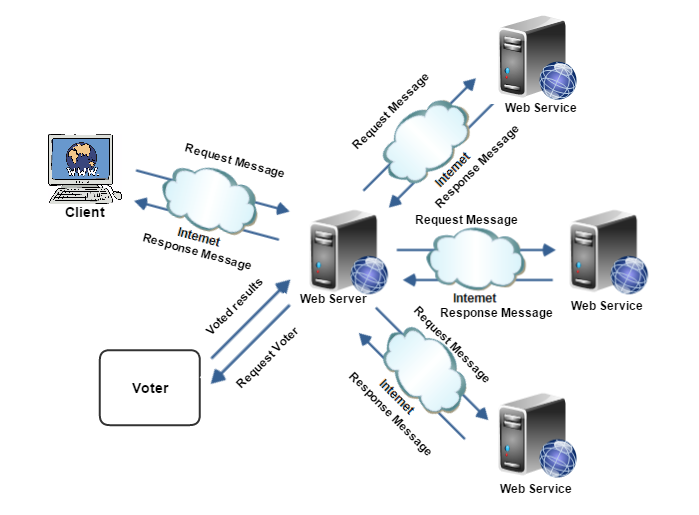
\includegraphics[keepaspectratio=true, scale=0.5]{Overview.png}
	\caption{Software Architecture of our Application}
	\label{architecture}
\end{figure}

To use the developed system, the user must make use of the \emph{Client Interface} provided, select the operation that he/she wants to invoke, input the necessary and requested parameters and  press the button \emph{"Calculate Insuline Dose"} to request the number of insulin units adequate for the parameters specified.

When the user presses this button a request is triggered to our \emph{Web Server} (hosting the \emph{Web Interface}). The \emph{Web Server} then randomly selects three \emph{Web Services}\footnote{From a previously generated list of \emph{Web Services}} and makes the desired request.

Then, for of the selected \emph{Web Services} the \emph{Server} either gets a response in feasible time or identifies the occurrence of a \emph{timeout} in the \emph{Web Service side}.

After receiving all the responses from the \emph{Web Services}, the \emph{Server} invokes the \emph{Voter}. The \emph{Voter System} collects all the responses from the \emph{Web Services} and selects the majority response which is presented to the user. In case a majority consensus can not be achieved the entire process is repeated, i.e., the request is sent to three different \emph{Web Services}  until there is no feasible time to retrieve the answer to the user. At that point a message is displayed in the \emph{Web Interface} reporting the situation (impossibility of obtaining a valid consensual final value).

\chapter{Web Service}
\label{web_service}

The present section is reserved to the description of the \emph{Web Service} implemented by our group. We start this chapter with a brief description of the technology used in the development of the service, deepening into the \emph{Web Method} implemented.

\section{Technology}

As requested in the work's assignment, the \emph{Web Service} was developed with the \emph{Java API for XML Web Services (JAX-WS)}. \emph{JAX-WS} is a very popular and useful technology for building \emph{Web Services} (and \emph{Web Clients}) using \emph{XML} for their communications.

Like many other \emph{Java EE APIs}, \emph{JAX-WS} makes use of the power of \emph{Java Annotations} to enable a quick, simple and easy development of \emph{endpoints} and \emph{Web Services}. Thanks to the annotations used, the complexity of many operations is hidden from the programmers, which eases and speeds up the development process.

In \emph{JAX-WS} a \emph{Web Service} consists in one class with a finite set of (public) \emph{Web Methods}, whose invocations by a client are accomplished using \emph{SOAP}, a\emph{XML-based protocol} that defines the envelope structure, encoding rules, and conventions for representing web service invocations and their responses, transmitted over the \emph{HTTP} protocol. Once the \emph{Web Service} is fully developed it should be hosted in a given \emph{URL}, along with a description of the services created and available, so that client applications know what services to invoke and how to invoke them. This description, called \emph{Web Services Description Language (WSDL)}, is generated and managed by the mentioned \emph{API}, and consists in a language written in \emph{XML} describing the service.

The development of the \emph{Client Application} is also very simple and straightforward: A client creates a local object that represents the service to invoke, called a \emph{Proxy}, and invokes all the desired methods\footnote{Also called \emph{Services}} through that same \emph{Proxy}. The \emph{JAX-WS API} offers a routine for generating the \emph{Proxy} based on the \emph{Web Services Description Language (WSDL)}, which means that, in the client side, the programmer does not need to generate or program in any way the \emph{Proxy}.

Besides providing a very simple, straightforward, quick and effortless way of developing \emph{Web Servers} and \emph{Clients} the \emph{JAX-WS API} also offers the platform independence of the \emph{Java} programming language, without making it a design constraint: A \emph{Non-Java Client} can access a \emph{Web Service} developed in \emph{C++} or any other programming language and vice versa.

\section{Web Methods}

    This section is dedicated to the description of each method available in the web-service. This methods were implemented based on the specifications indicated in the wording of the assignment. Once all the parameters are integers, the first step consisted in convert them to \emph{doubles} avoiding some possible \emph{rounding} errors. However, the result is rounded and converted to \emph{integer}.

\subsection{mealtimeInsulinDose}

    The aim of this method is to calculate the number of insulin units needed after a given meal.

    This method takes the amount of carbohydrate in a given meal, and returns
the number of units of insulin needed after that meal. The returned
number of units of insulin equals the carbohydrate dose plus the high
blood sugar dose, which are computed as follows.
    
    The carbohydrate dose equals the total grams of carbohydrates in the meal
divided by the amount of carbohydrate disposed by one unit of insulin,
corrected by taking into account the personal sensitivity to insulin.
This dose equals to:

$$carbohydrateAmount / carbohydrateToInsulinRatio / personalSensitivity \times 50$$

    The high blood sugar dose equals the difference between the pre-meal
blood sugar level and the target blood sugar level, divided by the
personal sensitivity to insulin. This equals $(preMealBloodSugar -
targetBloodSugar) / personalSensitivity$. The personal sensitivity
is can be explicitly indicated by the user or calculated using the $personalSensitivityToInsulin()$ method.

    In the special case when the target blood sugar level is greater than the
pre-meal blood sugar level, the return value of this method is zero (no
insulin).

\subsection{backgroundInsulinDose}

    This method calculates the total number of units of insulin needed between meals.
    
    The total insulin units required in one day equals $0.55 \times body
weight$ in kilograms. This method returns 50\% of that number, since
the background need for insulin, between meals, is around half of the
daily total.

\subsection{personalSensitivityToInsulin}

    This method is used to calculate the sensitivity to insulin based on the psychical activity level and blood sugar drop.
    
    One unit of insulin typically drops blood sugar by 50 mg/dl, but this
value depends on each individual's sensitivity and daily physical
activity. This method predicts the blood sugar drop (in mg/dl) that will
result from one unit of insulin, for a given physical activity level.

    To predict the blood sugar drop, this method accepts two arrays with
K samples of (physical activity level, blood sugar drop). The two arrays
must therefore have the same length. First, a simple linear regression
(least squares method) is performed to compute alpha and beta. Then, the
return value is $alpha + beta \times physicalActivityLevel$.

    The physical activity levels, including the ones in the array of samples,
and the blood sugar drop values are non-negative integers. The return
value of this method may be passed to $mealtimeInsulinDose()$
as a parameter.

\section{Deployment}

    The developed \emph{Web Service} was hosted in a virtual machine located at the Department of Informatics Engineering, under the url \url{liis-lab.dei.uc.pt}. The service was hosted in port $8080$, and the \emph{WSDL} can be accessed via \url{liis-lab.dei.uc.pt:8080/Server?wsdl}
    
    In fact, this virtual machine does not correspond to the set of virtual machines requested by the students of this course. This machine was being used by \emph{Joaquim Leitão} in a research project supervised by \emph{Prof. Alberto Cardoso}.
    
    Since it was not being used at the time this assignment was developed, we asked \emph{Prof. Alberto Cardoso} permission to use this machine, thus avoiding the unnecessary creation of another virtual machine. We would also like to take this opportunity to thank \emph{Prof. Alberto Cardoso} for his cooperation.

\chapter{Interface Application}
\label{interface_application}

    In this chapter, a detailed description of \emph{web application} will be made. Firstly, a general overview of application will be presented, followed by a more detailed explanation of \emph{client} and \emph{server} sides.

\section{Technology}

    \emph{Structs 2} was the chosen framework to implement the \emph{web application}. This is a very useful framework used to create MCV java web applications. Therefore, application is structured as follows:
    
    \underline{Views}:
    
    \begin{enumerate}
    \item \emph{index.jsp} - this is the initial view where all the calculation option are presented. The user is able to select one of the possible insulin calculation methods. After selected a given option, the input forms appears in the screen.
    \item \emph{meal\_personal.jsp} - in this method, the insulin sensitivity is calculated based on correlation between physical level and drop in blood sugar.
    \item \emph{meal\_standard} - similarly to the previous calculation method, all the parameters to needed to insulin calculation are requested to the user. However, in this case insulin sensitivity of the patient is explicitly indicated by him.
    \item \emph{background.jsp} - this view receives the patent's weight in order to calculate the background insulin dose.
    \item \emph{calculation\_results.jsp} - after all performed one of the considered insulin calculation method, this view presents the voted result. Additionally, the user can also check the results obtained in each web-service.
    
    
    
    \end{enumerate}
    
    \underline{Actions}:
    
    There is 3 distinct \emph{actions} to handle the each type of insulin dose calculation:
    
    \begin{enumerate}
    \item \emph{Background} - action called to calculate background insulin dose
    \item \emph{MealPersonal} - action called to firstly calculate patient's insulin sensitivity followed by insulin doses calculation.
    \item \emph{MealStandard} - action called to calculate background insulin dose based on a given insulin sensitivity
    \end{enumerate}
    
    All the considered actions are derived from a \emph{main action} named \textbf{User}. This action is responsible for the initialisation of a new \emph{bean} when it isn't already saved in the current session.
    
    \underline{Model}:
    
    Model is probably the most important part of this project. Web-services connections and voting system were implemented in this entity.
    
    There are 3 distinct main methods, one for each type of insulin dose calculation. Additionally, other methods were implemented to deal with web-service connections and voting system.

\section{Web Service Connection}

    In this section will be described the management of web-service connections and control of the service's response time.
    
    The first step consisted in implementing a new \emph{class}, named \emph{Client}, responsible for calling the web-service methods located at server-side. To call the web-service's methods an automatically generated \emph{proxy} was used, facilitating this task.
    
    Fig. \ref{FILHADAPUTA} shows an general overview of communication between \emph{model} and web-services. 
    
    \begin{figure}[H]
        \centering
        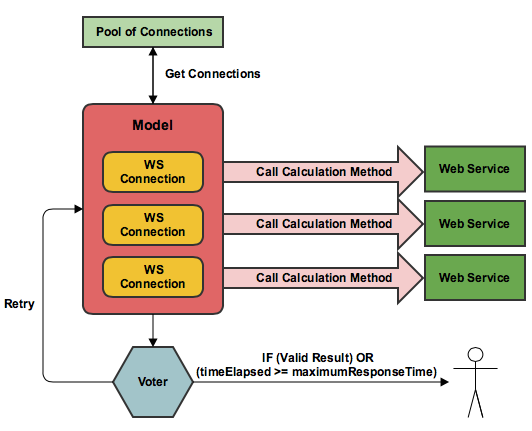
\includegraphics[width=\textwidth,height=\textheight,keepaspectratio]{webservice-2.png}
        \caption{Overview of communication between \emph{model} and web-services}
        \label{FILHADAPUTA}     
    \end{figure}
    
    Whenever the voter returns a valid result, the web-services used for the voting process are presented in the interface. Also the corresponded result of each one is shown.
    
\subsection{Pool of Connections}
    
    To manage the web-service's connections, a \emph{connections' pool} was implemented. This pool stores all the web-services URLs and allows the establishment of a new connection to a available web-service. So, when a \emph{model} method requires a new connection to a web-service, it calls the \emph{getNewConnection()} method from the pool of connections.
    
    Since a given web-service server can be offline, the pool stores a \emph{check-sum} indicating whether a given server is available or not. Note that a new connection corresponds to a new instance of \emph{Client} class.

\subsection{Limited Response Time}

    As requested, the user should receive the calculation result within a maximum period of 4 seconds. Therefore, some control mechanism were implemented to fulfil this requirement.
    
    The most trivial approach consisted in execute each request sequentially and setting an appropriate \emph{connection timeout} and \emph{request timeout} in web-service client. So a \emph{timeout exception} would be thrown by web-service client and that result will be not valid. However, some problems arises when using this approach. Thus, a different approach and possibly more elegant approach was adopted for this application.
    
    Firstly, all the web-services requests are running in parallel, meaning that each web-service's request is executed in an independent \emph{thread}. A \emph{maximum execution time} of each thread is defined being cancelled all the tasks that didn't finish within that time. When task doesn't finish, the result of that web-service is set with value -1, indicating that a \emph{timeout} occurred.
    
    However, when a given set of results are not enough to produce a valid result, the system establishes new connections and repeat the process while the elapsed time is less than 4 seconds.
    
\subsection{Error Handling}

    As described previously, a lot of exceptions can be thrown during a request of insulin calculation. To improve the robustness of the application, all the exceptions should be handled and notified to the user.
    
    The most important exceptions are related to the \emph{web-services' connections}. An exception is thrown whenever a given request thread could not achieve a valid result from the web-service. In this case, a new set of connections are established and the requests are performed again. However, when the elapsed time since user's request exceeds 4 seconds, the user is notified that something wrong happened.
    
    In order to simplify the error handling, when something wrong happens during a request the result is defined as -1. Thus, the user is redirected to the index page whenever a result equals to -1 is received.

\chapter{Voter}
\label{voter}

In this chapter we intend to perform a detailed description of the \emph{Voter System} that selects the final outcome to be presented to the user, as a result of a voting operation based on a series of answers provided by the selected \emph{N} versions of the \emph{Web Service}.

This is, in our opinion, the most challenging component of our system in a developer's point of view, due to its role and importance to our system. Therefore, in this chapter, we will also be addressing a formal verification of the developed voter, thus ensuring its correct behaviour.

\section{Technology}

Like the remaining components of our system, the \emph{Voter System} was developed in the \emph{Java} programming language and embedded in the \emph{model} structure of the \emph{Interface Application}, executed on the \emph{server side}.

As mentioned in chapter \ref{interface_application}, the \emph{Voter system} starts its execution after the results of the computations of the invoked \emph{Web Services} have been successfully received, or a \emph{timeout event} has been fired.

\section{Behaviour}

\subsection{Theory}

The basic and most basic principle behind any \emph{Voter System} is, given a series of values, determine which value is the most frequent and report it as the answer fort he given problem.

In the scenario of our application this would mean that, given the results of the computations from three or more \emph{Web Services}, the voter would identify the existence of a majority response\footnote{Corresponding to a value returned by the majority of the \emph{Web Services} requested}, selecting that value as the system's final response, to be presented to the application's user. Whenever there are no majority response, or when we have more than one majority response, the \emph{Voter} cannot make a decision regarding which value to present to the user, and as a consequence of that, the voting system fails\footnote{Which, as we have already addressed, will either trigger a new request for different \emph{Web Services} and the corresponding voting of the responses or stop the process, informing the user of the failure to satisfy his/hers request}.

Taking into account what we have just presented, and considering all the restrictions of the system to be developed we created a \emph{Voter System} with the behaviour that follows:

\begin{itemize}
\item The first step of the voter's execution consists in receiving all the results from the computations of the different \emph{Web Services} requested, including the ones that could not retrieve a result within the stipulated time window (For those in this situation the value $-1$ is considered).

\item The voter then proceeds to compute the number of occurrences of each of the results provided, taken into account the \emph{similarity restriction} imposed in the system's requirements\footnote{Any two values that only differ one unit must be considered the same in the voting mechanism. For example, for voting purposes, the values $3$ and $4$ are considered the same, but not the values $4$ and $6$}. In this procedure only the result with higher number of occurrences is stored, as well as the sequence of those elements (in case of multiple results with higher number of occurrences that information is also stored, as it will be needed further in the voting mechanism)

\item Once the voter knows which results have the higher number of occurrences it can make a decision regarding the result to be selected: If we only have one sequence with higher number of occurrences we compute its median and take that value as the result of the voter. Otherwise, if we have more than one sequence in these conditions we cannot make any decision regarding the majority response of the requested \emph{Web Services}, thus an invalid value ($-1$ in our implementation) is selected and returned to the \emph{Interface Application}, which will identify it and inform the user of the inability of the system to satisfy the requested operation
\end{itemize}

\subsection{Example}

Even though we consider the behaviour of the voter described in the previous subsection to be quite simple, we believe that providing the reader with a simple example of its behaviour and operation mode will ease its understanding. Therefore, in this subsection an example of a possible scenario in our application is presented and the behaviour of the \emph{Voter} is explained.

Consider that, in our application, we are making requests for a given service to $7$ \emph{Web Services}, each with its own implementations. Consider also that the results produced by those \emph{Web Services}, after being sorted are the following: $[1,1,2,3,4,6,8]$.

If we compute the number of occurrences for each element, as previously described we would get the following:

\begin{itemize}
\item Element $1$ with $3$ occurrences, in the sequence: $[1,1,2]$
\item Element $2$ with $4$ occurrences, in the sequence: $[1,1,2,3]$
\item Element $3$ with $3$ occurrences, in the sequence: $[2,3,4]$
\item Element $4$ with $2$ occurrences, in the sequence: $[3,4]$
\item Element $5$ with $2$ occurrences, in the sequence: $[4,6]$
\item Element $6$ with $1$ occurrence, in the sequence: $[6]$
\item Element $8$ with $1$ occurrence, in the sequence: $[8]$
\end{itemize}

Please note that, in this step, we can compute sequences of elements that were not produced by any \emph{Web Service}. This is simply due to the fact that, in our system, we need to take into account the similarity between values that only differ one unit.

Given the results obtained in the presented scenario, the voter would select the value $2$ as its answer (and thus it would be presented to the user) since it is the element with the higher number of occurrences.

If, for example, the results computed from the \emph{Web Services} were  $[1,2,3,4,6,8,11]$, then a majority response would not have been achieved (since we would have three elements with the higher number of occurrences) and the voter would need to report that situation to the application, by returning the value $-1$.

\section{Implementation}

    To implement the behaviour proposed and described in the previous section we implemented two methods, \emph{voter} and \emph{median}, added and used in the \emph{Model} of the \emph{Interface Application}. In the remainder of this section we provide the reader with some detail regarding these two methods.
    
\subsection{voter}

With the \emph{Voter} method we seeked to implement the process described in the previous section regarding the identification of a majority response among the \emph{Web Services} requested. To achieve this we made use of the implementations of some data structures in \emph{Java}, like the \emph{ArrayList} and the \emph{HashMap}.

In this method we sort the results received from the \emph{Web Services}, and create a list of \emph{buckets}, where each \emph{bucket} is used to store the occurrences of each of the results provided, taken into account the \emph{similarity restriction} imposed in the system's requirements. While we are creating this list we store the size of the biggest sequence registered so far and a flag that tells us if our biggest sequence is unique\footnote{This flag is implemented as a \emph{Boolean} variable}.

Once this procedure is finished we simply need to check for the value in the mentioned flag: If its value indicates a unique sequence then we can move to the next step in the execution, computing the median of that sequence. Otherwise we can simply terminate the voting process, since no majority was achieved.

\subsection{median}

As the name suggests, this method simply computes and returns the median of a given set ordered of values, used to determine the \emph{Voter's} response in a scenario where a majority response was achieved.

This computation is pretty straightforward: First we need to check if the number of elements is even or odd. In the latter case we take the middle element of the set as the median, and in the first case we need to compute the average of the two middle elements, rounding it to the smallest closest integer.

We decided to round the answer to the smallest closer integer because not only we felt that, in a real situation, if we are unable to administrate the exact number of insulin units the patient needs, then it is better to administrate a slightly smaller amount than an amount of insulin higher than what is recommended. In fact, in a real situation, injecting the patient with a smaller insulin dose than what he/she needs can lead to a state of \emph{hypoglycemia}, which is better for the patient than the opposite state, \emph{hyperglycemia}.

In fact, if one reflects on our purposed implementation of the \emph{Voter System}, one can argue that it may not be the best solution for the problem we are addressing, at least not at a conceptual level.

Indeed, we agree that the creation of a class to represent the \emph{Voter} would be, conceptually, more accurate and could even ease the re-usability and maintenance of our code and application. However, we made the decision to keep our \emph{Voter} implementation as presented, given its simplicity: Even if we created a class to model the behaviour of the \emph{Voter} we felt that the added value that it could bring to our application was not very high given the current \emph{Voter's} implementation.

Nevertheless, we want to stress the fact that, in a real application we would probably had chosen to implement a class to model the behaviour of the \emph{Voter}, since it would provide us with a better abstraction and could ease the implementation of new functionalities in the \emph{Voter}.

\section{Formal Verification}

Given the importance of the \emph{Voter} in the application developed (after all, it is the voter who determines what the system's response should be) there is a need and an interest in formally verifying the behaviour of this system: If we can guarantee that our \emph{Voter} is working according to a given agreeable model, and that the model in question is formally correct, then if the implementation of that entity is done strictly according to that model, we can be sure that that particular entity will not misbehave. This is, obviously, very important in software  quality and dependability.

To formally verify the \emph{Voter} described, we created a model in the \emph{Promela} process modelling language\footnote{Whose intended use is to verify the logic of parallel systems}. Having built the model we can then use \emph{SPIN}\footnote{A very popular tool used for verifying the correctness of distributed software models} to verify the correctness of the model by simulating all the possible combinations of executions in our model.

Given the fact that \emph{Promela} only allows the usage of a very basic set of data types, thus not supporting most of the data structures available in the \emph{Java} programming language, we needed to perform some simplifications in the model produced, when compared to the \emph{Java} implementation of the \emph{Voter}:

\begin{itemize}
\item For starters, in the produced model we do not execute in any way a call for a \emph{Web Service}. We simply simulate its behaviour by randomly generating an output value from a previously defined output range.

\item Even though we did not execute or implemented any of the \emph{Web Services}, we decided to model the occurrence of \emph{timeout events}, due to their importance in the system and the complexity they add to the entire system. In the \emph{Promela} model such events are simulated through the execution of an instruction consisting only in a variable that has the value $0$\footnote{In \emph{Promela} the value $0$ is mapped to the statement $false$, and the execution of instructions containing only a \emph{false value} (Like the execution of the instruction $(0);$ or $(false);$) result in the blocking of the process that is attempting to execute those instructions}

\item We have also performed a series of \emph{assertions} throughout our model, to detect invalid execution states that, if reached, would confirm an improper implementation of the \emph{Voter} according to what we defined in our model\footnote{For example, if at any given point in the execution we determine that the \emph{Voter} is not able to make a decision, then before the execution of the model finishes we are asserting that, in fact, the \emph{Voter} reached that conclusion}.

\item Since we found no reliable way of measuring the execution time in our model we decided to model the maximum response time for our system (which, in our scenario was of $4$ seconds) in a maximum number of invocations that can be made to the \emph{Web Services}. Even though we understand the differences between these two approaches, we do believe that the solution proposed is an acceptable abstraction that can be considered in our model. 
\end{itemize}

The \emph{Promela} code developed to model the behaviour of the \emph{Voter} will be provided along with this report so the reader can, if that is his/hers wish, verify and simulate the model we created.

The model presented in this section, which code is provided along with this report, was exhaustively checked and verified with \emph{SPIN} and in all the tests and verifications performed no assertion or error was triggered, and the behaviour showed by the \emph{Voter} was, in our opinion, according to what is expected in this assignment: Whenever no majority was founded the \emph{Voter} did not select any value; And when a majority was, in fact, achieved the \emph{Voter} selected the median of the elements forming that majority as its result.

\chapter{Conclusion}
\label{conclusion}

    In summary, the first step of this work consisted of implementing a version of web-service following the structure previously defined. Afterwards, a \emph{Web Server} was implemented as well as a voting system for the final result. Finally, this voter was formally verified using the \emph{PROMELA} programming language.
    
    In our opinion, N-Version programming is a very useful process for the implementation of critical systems. Furthermore, the voting system is clearly the main part of this software process. Therefore, a strict set of criteria were defined to produced a reliable result to the patient. However, we consider that other criteria should be defined to avoid some undesired situations.
    
    According to the implementation proposed in this work, considering the following set of results: [1,1,1,2,6,6,6] the voted result is 1. However, this is an ambiguous result given that we consider that is not possible to reach a clearly majority with this set of results: We simply have more \emph{1's} and \emph{6's} because we considered results that differ one unit to be the same, but even considering this we do not have a clear consensus among the selected \emph{Web Services}. A hypothetical alternative could be to check the result with an another set web-services, used specifically for these types of situations.
    
    It is also worth mentioning that, while we understand the importance and value that a formal verification of a software entity adds to the quality, dependability and reliability of any system, we still struggled with this task in our assignment. This was mostly due to the restrictions imposed by \emph{Promela} (which only allows programmers to use an adapted and very restrict set of the \emph{C} programming language, making it extremely difficult for us to model the interactions between the different entities in our system, as we would liked to have done, instead of just modelling the voting operation.
    
    We also feel that we should have found a better way to model the behaviour of each \emph{Web Service}, as simply generating random values in a previously defined range does not feel very realistic and adequate. However, we were unable to come up with a better alternative, and ended up with the presented model. Probably one of our biggest disappointments in this work was exactly the fact we felt we were not taking full advantage of both the \emph{Promela} and \emph{SPIN} tools.
    
    Nevertheless, we were still able to model and test some interesting behaviours,like the similarity between values that differ only one unit (Thus simulating differences in rounding operations made in different \emph{Web Services}), which we believe to be an important aspect to take into account in any \emph{Voter} system.
    
    Still, building the model for our voter turned out to be probably one of the most useful tasks we performed in this work, since we made us think and rethink our approach to the implementation of this system, enabling us to have a better understanding of what should the \emph{Voter} do, and how it should be accomplish, which is, after all, one of the goals of this modelling process.

\end{document}
